\documentclass[12pt,letterpaper,boxed,cm]{hmcpset}

\usepackage[margin=1in]{geometry}
\usepackage{mathtools}
\usepackage{mathrsfs}
\usepackage{graphicx}
\usepackage{soul}
\usepackage{cases}

\name{A GIRL HAS NO NAME}
\class{Computer Science 81}
\assignment{Homework 4}
\duedate{2/14/17}

\newcommand{\pn}[1]{\left( #1 \right)}
\newcommand{\abs}[1]{\left| #1 \right|}
\newcommand{\bk}[1]{\left[ #1 \right]}
\newcommand{\set}[1]{\left\{#1\right\}}
\newcommand{\ra}[0]{\rightarrow}
\newcommand{\cp}[0]{~\vdash~}


\begin{document}
\problemlist{1, 2, 3, 4}

\begin{problem}[1.]
    \textbf{Sequences} [20 points]\\
    We say that an infinite sequence $a_0,a_1,a_2,a_3,\ldots$ of real numbers has the limit $L$ if \ul{for every strictly positive number $\epsilon$, there is a natural number $n$ such that all the elements $a_n,a_{n+1},a_{n+2},\ldots$  are within distance $\epsilon$ of the value $L$.} In this case, we say that $\lim a = L$.
    \begin{enumerate}
        \item [A.] [3 points] Express the condition that $\lim a = L$ as a formula of predicate logic. You may use typical math functions and relations like $>$ or $\in$ (but not ``$\ldots$'').   Your formula should only have two free variables: $a$ and $L$.
        \item [B.] [9 points] For any two infinite sequences $a = a_0,a_1,a_2,\ldots$ and $b  =  b_0,b_1,b_2,\ldots$ then we define their \ul{sum} $a+b$ to be an infinite sequence $c_0,c_1,c_2,c_3,\ldots$ such that $c_i = a_i + b_i$ for every $i\ge0$. Carefully and convincingly prove (in “mathematical English,” not Jape!) that if we have two infinite sequences with $\lim a = L$  and  $\lim b = M$  then $\lim (a+b) = (L+M)$. 
        \item [C.] [5 points] Identify 5 places in your proof where you took a step corresponding to a natural deduction rule, explicitly or implicitly. Each place should correspond to a different natural deduction rule.  (If you can’t do this fairly easily, you may need to reconsider the structure of your proof.)
        \item [D.] [3 points] Your proof almost certainly used (perhaps implicitly) well-known mathematical “facts” about natural numbers or real numbers.  These “facts” are just small theorems that are so well-known that they can be used in proofs without comment. Use predicate logic formulas to specify three theorems you used. (You don’t need to provide proofs them, but they should all be true formulas with no free variables.)
    \end{enumerate}
\end{problem}

\begin{solution}
    \vfill
\end{solution}
\newpage

\begin{problem}[2.] 
    \textbf{"You are in a Maze of Twisty Little Passages, All Alike"} [34 points]\\
    \begin{center}
        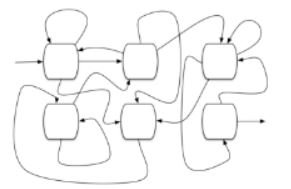
\includegraphics{01.jpg}
    \end{center}
    Suppose we have designed a maze consisting of rooms connected by (simple or complex) \ul{one-way} passages. One room is designated as the starting point (because it has the entrance), and another room is designated as your goal (because it has the maze exit). \\

    If we’re designing a maze, we could make a plan with a finite number of rooms or even an infinite number of rooms! We say that a maze is \emph{finite} when it has a finite number of rooms.\\

    A \emph{path} in the maze is specified by a (finite, possibly-empty) ordered list/sequence of the passages traversed, beginning at the room designated as the maze’s starting point. \\
    A path is a \emph{solution} if traversing the specified passages in order would get you from the starting room to the goal room.  The \emph{length} of a path $p$ is written $\abs{p}$, and is just the number of passages traversed in the path. (Note that when doing “maze theory”, we don’t care about how far apart rooms are. Each passage in the path, no matter how long, adds 1 to the length.)
    \begin{enumerate}
        \item [A.] [1 point] Suppose we have a maze has exactly 19 rooms. You begin at its starting point and then wander through 27 (one-way) passages. What can you conclude about the rooms you visited, and why?
        \item [B.] [4 points] Here is a theorem about all finite mazes (mazes with a finite number of rooms):\\

        \textbf{Theorem 1:} \emph{For every finite maze there is a number $n$ such that: every path $s$ through the maze with length $n$ or more contains \ul{at least one loop that starts and ends within the first $n$ steps.}}\\

        \emph{Briefly} explain why Theorem 1 is true.  (E.g., how can we find such a number $n$? Why must paths at least that long contain a loop as described?)
    \end{enumerate}
\end{problem}
\newpage
\begin{problem} [2. cont.]
    \begin{enumerate}
        \item [C.] [1 point] How can Theorem 1 be true for the following finite maze, which has no loops? Explain briefly.
        \begin{center}
            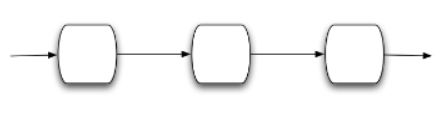
\includegraphics{02.JPG}
        \end{center}
        \item [D.] [3 points] Here is a more sophisticated theorem about all finite mazes:

        \textbf{Theorem 2:} \emph{For every maze $M$, if $M$ is finite then \ul{there is a natural number $n$ such that: whenever there is a \textbf{solution} of length $\abs{s} ≥ n$, then $\abs{s} = a + b + c$ for some natural numbers $a\ge0$ and $b>0$ and $c \ge 0$ such that (1) $a+b \le n$ and (2) there is a solution to the maze of length $a + kb + c$ for every integer $k \ge 0$.}}\\

        Express the underlined phrase as symbolic predicate logic (and standard math notation such as $+$ and $=$. You may also use the predicate \textbf{Solution}$(M,s)$ to mean that $s$ is a solution to maze $M$. Your formula should have $M$ as its only free variable.
        \item [E.] [9 points] Prove Theorem 2 (remembering to use complete sentences). Your proof can make use of Theorem 1, and should explain how suitable natural numbers a, b, and c can be found (when they exist).
        \item [F.] [3 points] Identify 3 places in your proof of Theorem 2 that correspond (at least implicitly) to natural deduction steps.
        \item [G.] [3 points] Since $\phi \ra \psi$ is equivalent to $\neg\psi\ra\neg\phi$, we know that \ul{if} a maze $M$ satisfies the \ul{negation} of the formula in part D, then we can be sure $M$ is \ul{not} finite. 

        Negate the formula in D and then find an equivalent formula where the $\neg$ has been pushed “inwards” as far as possible. [For example, you can replace $\neg\exists n\ldots$ by $\forall n. \neg\ldots$, and so on. It might be helpful to push negation into conjunctions like $\neg\pn{\phi\land\ldots\land\psi\land\theta}$ as $\pn{\phi\land\ldots\land\psi \ra \neg\theta}$ instead of DeMorgan’s $\pn{\neg\phi\lor\ldots\lor\neg\psi\lor\neg\theta}$.]
        \item [H.] [9 points] Suppose maze $M_a$ has the following property: for every integer $i \ge 1$ there is a solution of length $2^i$, and there are no solutions of other lengths. Carefully show how we can use Part G (and logical argument) to prove that maze $M_a$ \ul{cannot} be finite.
        \item [I.] [1 point] Suppose we have a maze $M_b$ that satisfies the formula you wrote for Part \textbf{D} (not G!). Can we use Theorem 2 (and logical argument) to prove that maze $M_b$ \ul{is} finite, or to prove that $M_b$ \ul{is not} finite? Justify your conclusion.
    \end{enumerate}
\end{problem}

\begin{solution}
    \vfill
\end{solution}
\newpage

\begin{problem}[3.]
    \textbf{Conclusion} [1 easy point]\\
    Please wait until you’re done with the rest of the assignment to answer this quick survey:
    \begin{enumerate}
        \item [A.] How long (in hours) did you spend working on this assignment?
        \item [B.] What was the most interesting thing you learned while answering these problems? (We’re sure there was \emph{something} you learned.)
    \end{enumerate}
\end{problem}

\begin{solution}
    \vfill
\end{solution}

\end{document}

